\acs{blam} is an open\hyp{}source \acs{lidar} based real\hyp{}time \acs{3d} \acs{slam} software package. Developed in 2016 by Erik Nelson from the \ac{bair} laboratory. The software is build in a \acs{ros} environment, containing two \acs{ros} workspaces. \cite{github_blam}

Because of its outdated dependencies and the difficulty of installation, there was no implementation possible of \acs{blam} in this project. \acs{blam} has \acs{ros}, \acs{gtsam}, and Boost as a dependency. The algorithm looked promising, but it does not support a camera as a sensor for visual odometry.

\begin{figure}[!h]
  \centering
  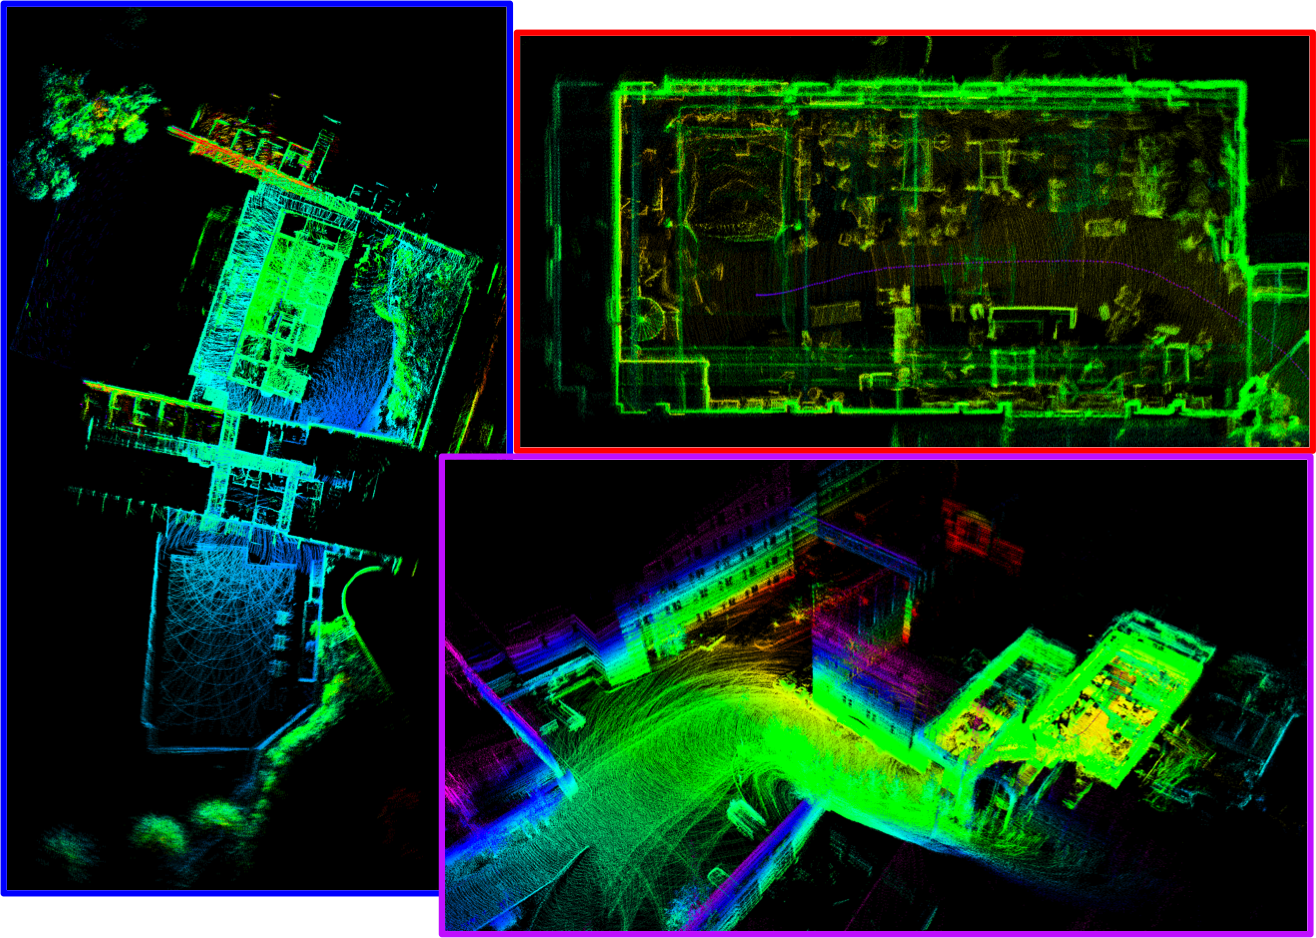
\includegraphics[width=\linewidth]{images/blam.png}
  \caption{BLAM! example \cite{github_blam}}
\end{figure}